\chapter{MOC Parameter Sensitivity Studies}
\label{chap:moc-sensitivity}

In this chapter, sensitivities to both spatial mesh refinement and \ac{MOC} ray refinement are studied in detail. Radial sensitivities, which have been studied extensively in 2D \ac{MOC} are first discussed. Then, the axial sensitivities are studied. Both radial and axial sensitivities include mesh refinement as well as ray refinement studies with the OpenMOC linear source solver on BEAVRS geometries. These studies all involve models without control rod insertions. The axial sensitivity studies are then repeated for the case of a single assembly with a partially inserted control rod. In addition, the sensitivity of convergence to \ac{CMFD} parameters and domain decomposition is also studied. This chapter concludes by presenting the chosen parameters to accurately and efficiently conduct \ac{PWR} simulations with 3D \ac{MOC}. The uninterested reader can skip to the conclusion of this chapter where the chosen parameters are presented.

%In Section~\ref{sec:axial-sensitivity-rodded}, the axial sensitivity study is repeated for the case of a single assembly with a partially inserted control rod. In Section~\ref{sec:flat-linear-comparison}, a comparison of flat and linear source solvers is presented for fixed \ac{MOC} ray and mesh refinement. Section~\ref{sec:cmfd-convergence-params} then focuses on the sensitivity of acceleration to \ac{CMFD} parameters. Whereas other sections focus on solution accuracy, the analysis in Section~\ref{sec:cmfd-convergence-params} studies the effect on convergence rate. In Section~\ref{sec:domain-decomposition-convergence}, the sensitivity of convergence to domain decomposition is analyzed. Lastly, Section~\ref{sec:sensitivity-conclusion} concludes the section by presenting the chosen parameters to accurately and efficiently conduct \ac{PWR} simulations with 3D \ac{MOC}. The uninterested reader can skip to the conclusion of this chapter where the chosen parameters are presented.

%%%%%%%%%%%%%%%%%%%%%%%%%%%%%%%%%%%%%%%%%%%%%%%%%%%%%%%%%%%%%%%%%%%%%%%%%%%%%%%%
\section{Radial Sensitivity}
\label{sec:radial-sensitivity}

Due to extensive experience with 2D \ac{MOC}, the radial parameters required to achieve sufficient accuracy -- both in mesh and ray refinement -- are relatively well known. These requirements for linear source were thoroughly studied by Ferrer~\cite{ferrer2012linear}. Based on these studies and CASMO-5 default parameters~\cite{rhodes2006casmo}, the expected radial parameters needed to achieve a sufficiently accurate solution are given in Table~\ref{tab:expected-radial-params}. Each of the parameters listed in the table will be thoroughly discussed and undergo a refinement study.

\begin{table}[ht]
	\centering
	\caption{Expected radial MOC parameters to sufficiently resolve the \ac{MOC} fission distribution using a linear source approximation}
	\medskip
	\begin{tabular}{lc}
		\hline
		Number of Rings in Fuel and Moderator & 1 \\
		Number of Sectors in Fuel & 4 \\
		Number of Sectors in Moderator & 8 \\
		Number of Sectors in Guide Tubes & 8 \\	
		Radial Ray Spacing & 0.05 cm \\
		Number of Azimuthal Angles & 64 \\
		Reflector Mesh & $3 \times 3$ cells per pin-cell mesh \\
		\hline
	\end{tabular}
	\label{tab:expected-radial-params}
\end{table}

\subsection{Core Radial Mesh Refinement}

First, the radial mesh within the core is studied. The core is composed of a lattice of assemblies. Therefore, the mesh refinement can be studied on a single assembly model. Since the axial dimensions should not largely impact the radial sensitivity, the short single assembly model is used, which is a 10 cm tall single assembly region without any grid spacers and reflective boundary conditions placed in both axial directions. This model is described in detail in Appendix~\ref{app:short-single-assembly}. This problem is simulated with the \ac{MOC} ray parameters given in Table~\ref{tab:rad-mesh-refinement-params}. These parameters are quite fine in the radial direction in order to accurately test the impact of the radial mesh. In the axial direction, the source height and axial ray spacing are quite coarse as the problem is uniform axially with no physical axial flux shape.

\begin{table}[ht]
	\centering
	\caption{MOC ray parameters for core mesh refinement studies}
	\medskip
	\begin{tabular}{lc}
		\hline
		Radial Ray Spacing & 0.025 cm \\
		Number of Azimuthal Angles & 128 \\
		Axial Ray Spacing & 3.0 cm \\
		Number of Polar Angles & 10 \\
		Axial Source Height & 10.0 cm \\
		\hline
	\end{tabular}
	\label{tab:rad-mesh-refinement-params}
\end{table}

The radial profile of the fission rate distribution of the short assembly fuel rods is shown in Figure~\ref{fig:short-assembly-radial}. The fission rates are calculated by running OpenMOC on the model with fine radial mesh. The radial distribution is formed by integrating the fission rates of all materials within each pin-cell.

\begin{figure}[h!]
	\centering
	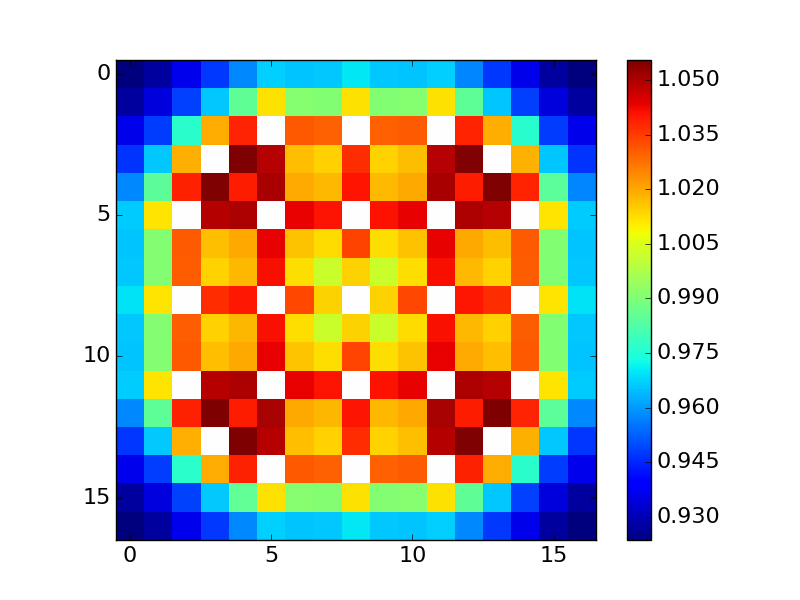
\includegraphics[width=0.7\linewidth]{figures/results/rr-plots/short-assembly-radial.png}
	\caption[]{The fission rate distribution over pin-cells for the short single assembly model.}
	\label{fig:short-assembly-radial}
\end{figure}

Typically, pin-cells are discretized into rings and sectors, as presented in Figure~\ref{fig:rings-sectors}. Ring divisions help to capture radial variation within the pin-cell and sector divisions help to capture azimuthal variation.

\begin{figure}[h!]
	\centering
	\begin{subfigure}{0.3\textwidth}
		\centering
		
\includegraphics[width=\linewidth]{figures/simp_fuel_pin.png}
		\caption{}
		\label{fig:rings-sectors-a}
	\end{subfigure}
	\begin{subfigure}{0.3\textwidth}
		\centering
		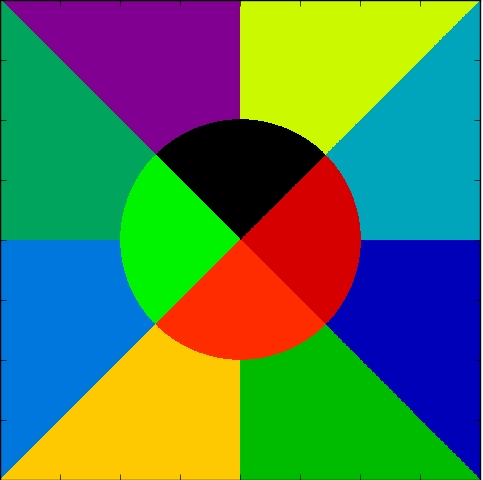
\includegraphics[width=\linewidth]{figures/sector_discr.jpg}
		\caption{}
		\label{fig:rings-sectors-b}
	\end{subfigure}
	\begin{subfigure}{0.3\textwidth}
		\centering
		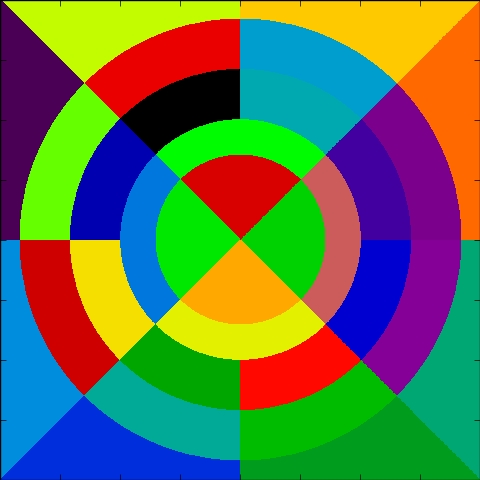
\includegraphics[width=\linewidth]{figures/ring_sector_discr.jpg}
		\caption{}
		\label{fig:rings-sectors-c}
	\end{subfigure}
	\caption[]{A simplified pin-cell (a) of just moderator and homogenized fuel is discretized (b) into 8 sectors in the moderator and 4 sectors in the fuel and further discretized (c) into 2 rings in the fuel and 3 rings in the moderator.}
	\label{fig:rings-sectors}
\end{figure}

While the illustration in Figure~\ref{fig:rings-sectors} only shows fuel and moderator regions, realistic pin-cells contain fuel, gap, clad, and moderator. For mesh refinement, ring divisions are never added in gap and clad regions since they are so thin. In our studies, the sector divisions within fuel is also applied to the associated gap and clad regions.

Since both fuel pins and guide tubes exist in fuel assemblies, there are three main zones of interest that could be independently discretized: fuel pins, guide tubes, and moderator.

\subsubsection{Ring Divisions}

%First, ring divisions are studied. The number of rings is counted by the number of \texttt{ZCylinder} surfaces bounding the region. For instance, 1 ring implies no further discretization in the regions. 

%For fuel rods and guide tubes, these rings divide the regions by creating concentric \texttt{ZCylinder} surfaces inside the rod such that the volume of all regions are equal. For moderator regions, \texttt{ZCylinder} objects are created outside the rod in concentric circles such that the distance between the surfaces is equal. Since there is no bounding outer \texttt{ZCylinder}, a virtual bounding \texttt{ZCylinder} is created with volume equal to that of the pin-cell.

First, ring divisions are studied. The sensitivity studies of ring divisions are shown in Table~\ref{tab:ring-sensitivity}. All fission rate errors are for a pin-wise mesh. Relative error in this thesis is always computed as
\begin{equation}
\textit{relative error} = \frac{\textit{trial} - \textit{reference}}{\textit{reference}}.
\end{equation}
For all cases, the expected radial mesh parameters are used unless otherwise specified. For each zone, a separate parameter refinement is conducted using 1, 2, and 3 rings. The 3 ring case is always chosen as the reference. For the other radial mesh parameters, expected parameters are used (1 ring in all regions with 4 sectors in fuel and 8 sectors in the moderator and guide tube).

\begin{table}[ht]
	\centering
	\caption{MOC sensitivity to mesh refinement by radial rings in fuel, guide tube, and moderator regions}
	\medskip
	\begin{tabular}{c|c|c|c|c|c}
		\hline
		 & No. of  & & $k_{\textit{eff}}$ & \ac{RMS} Fission & Max Fission \\
		Region  & Rings & $k_{\textit{eff}}$ & Error & Rate Error & Rate Error \\
		\hline
		Fuel & 1 & 1.21568 & 0.9 pcm  & 0.002 \% & 0.003 \% \\
		Fuel & 2 & 1.21569 & 0.4 pcm  & 0.001 \% & 0.002 \% \\
		Fuel & 3 & 1.21569 & -- & -- & -- \\
		\hline
		\hline
		Guide Tube & 1 & 1.21569 & 0.1 pcm & 0.002 \% & 0.004 \% \\
		Guide Tube & 2 & 1.21569 & <0.1 pcm  & 0.002 \% & 0.004 \% \\
		Guide Tube & 3 & 1.21569 & -- & -- & -- \\
		\hline
		\hline
		Moderator & 1 & 1.21569 & 4.7 cm  & 0.003 \% & 0.007 \% \\
		Moderator & 2 & 1.21564 & -0.3 pcm  & 0.002 \% & -0.004 \% \\
		Moderator & 3 & 1.21564 & -- & -- & -- \\
		\hline
	\end{tabular}
	\label{tab:ring-sensitivity}
\end{table}

These results show very little sensitivity. With a linear source approximation, gradients can be accurately captured without further radial discretization, causing ring divisions to be less important. Therefore, all tests in this study do not use ring discretizations. 

\subsubsection{Sector Divisions}

Next, azimuthal sector discretization in analyzed. Since these  discretizations largely account for azimuthal differences rather than radial gradients, they might still be needed with a linear source approximation. Again, the three regions (fuel, guide tubes, and moderator) are analyzed separately. Recall that gap and clad are discretized into the same number of sectors as the rod they surround.

For all of the cases, the \ac{RMS} and maximum fission rate error is inconsequential, similar to that observed with discretization by rings.  The maximum error occurred when comparing a case without any sector discretization for moderator, in which the \ac{RMS} fission rate error was 0.1\% and the maximum fission rate error was 0.3\%, which are both fairly low. However, the effect on the eigenvalue $k_{\textit{eff}}$ is substantial. Therefore, the results for sector discretization focus on the impact on eigenvalue.

Similar to the approach taken for discretizing by rings, all mesh parameters are taken to be the expected parameters except the parameter being tested. All error estimates are formed relative to 16 sectors. Figure~\ref{fig:comb-sectors} shows the sensitivity to the sector discretization of fuel, guide tubes, and moderator.

\begin{figure}[h!]
	\centering
	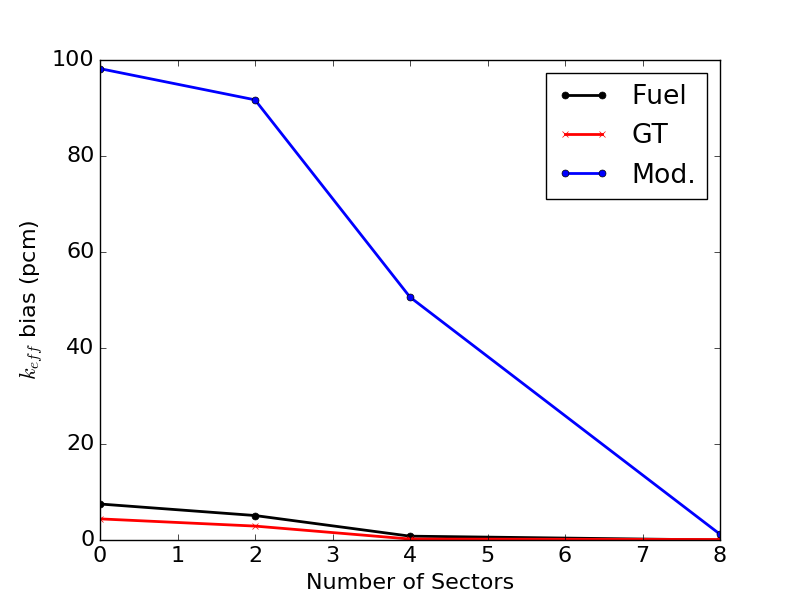
\includegraphics[width=0.7\linewidth]{figures/results/sensitivity/comb_sectors.png}
	\caption[]{The bias in eigenvalue $k_{\textit{eff}}$ decreasing as the number of sector discretizations increased in fuel rod, guide tube, and moderator regions.}
	\label{fig:comb-sectors}
\end{figure}


These results show the moderator region is again the most sensitive. After 8 sectors in the moderator and 4 in fuel and guide tubes, very little sensitivity is observed. This would imply that requiring 8 sectors in the guide tubes may be excessive, but guide tubes are relatively sparse throughout the core so the increased discretization has little impact on computational requirements. Therefore, in order to be conservative, 8 sectors remains the choice for guide tube discretization.

\newpage
\subsection{Reflector Radial Mesh Refinement}

Ring and sector discretizations form a well-defined mesh refinement within the core. However, for full core problems, the radial water reflector also needs to be discretized. To simplify the sensitivity study, a uniform global mesh is overlaid across the reflector regions. In addition, the discretization is chosen to align with \ac{CMFD} cell boundaries. In OpenMOC, \ac{CMFD} cell boundaries naturally create mesh discretizations as cells are split at the mesh boundaries. Since a pin-cell width uniform \ac{CMFD} mesh is chosen for acceleration of BEAVRS problems, the reflector is naturally discretized into pin-cell-sized regions. The radial mesh refinement then takes the form of a uniform mesh discretization within a pin-cell-sized region in which a square mesh refinement is chosen. Since each assembly contains a lattice of $17\times 17$ cells and an assembly width is $\approx 21.5$ cm (when including inter-assembly gap), the radial reflector mesh refinement takes the form of an $N \times N$ discretization of each 1.264 cm $\times$ 1.264 cm region within the reflector.

In order to conduct radial reflector mesh refinement sensitivity studies, a full core model is necessary. However, the full 3D BEAVRS model is computationally demanding. Therefore, the 2D BEAVRS model described in Appendix~\ref{app:beavrs-2D} is chosen. This model represents a radial cut of the full core BEAVRS geometry that has been extruded 10 cm in height with reflective boundary conditions placed on the top and bottom of the geometry. With the height greatly reduced from the full 3D model, the computational requirements are far less. In addition, since this model contains no axial variation, the radial sensitivity can be tested more directly. The \ac{MOC} parameters used in this sensitivity study are presented in Table~\ref{tab:rad-ref-refinement-params}.


\begin{table}[ht]
	\centering
	\caption{The MOC parameters used in the radial water reflector mesh refinement studies}
	\medskip
	\begin{tabular}{lc}
		\hline
		Radial Ray Spacing & 0.1 cm \\
		Number of Azimuthal Angles & 32 \\
		Axial Ray Spacing & 1.5 cm \\
		Number of Polar Angles & 10 \\
		Axial Source Height & 2.0 cm \\
		\hline
	\end{tabular}
	\label{tab:rad-ref-refinement-params}
\end{table}

The radial profile of the fission rate distribution of the 2D BEAVRS model is shown in Figure~\ref{fig:beavrs-2d-radial}. The fission rates are calculated by running OpenMOC on the model with fine radial mesh in the reflector.

\begin{figure}[h!]
	\centering
	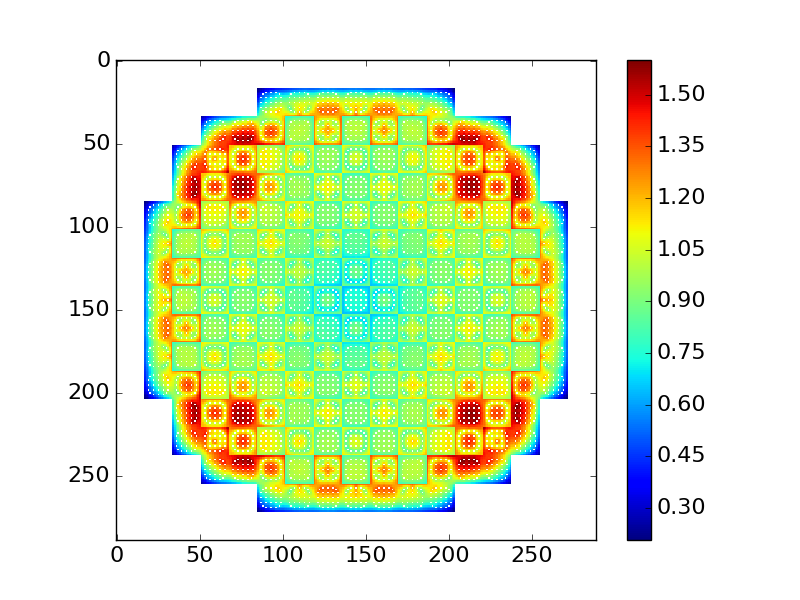
\includegraphics[width=0.9\linewidth]{figures/results/rr-plots/beavrs-2d-radial.png}
	\caption[]{The fission rate distribution of pin-cells for the 2D BEAVRS model.}
	\label{fig:beavrs-2d-radial}
\end{figure}

The results of the sensitivity study are presented in Figures~\ref{fig:rad-ref-pcm} and \ref{fig:rad-ref-fr} for eigenvalue and fission rate, respectively. All sensitivities are compared to a reference solution which uses a $5\times 5$ radial reflector mesh discretization. The results show little sensitivity to the reflector mesh, likely since the linear source approximation is able to accurately capture gradients. At the expected $3 \times 3$ reflector mesh refinement, the eigenvalue bias is below 1 pcm and all relative fission rate errors are below 0.1\%. Therefore, the  $3 \times 3$ radial reflector mesh discretization is sufficient to accurately resolve the solution and is chosen for all further studies and results.

\begin{figure}[h!]
	\centering
	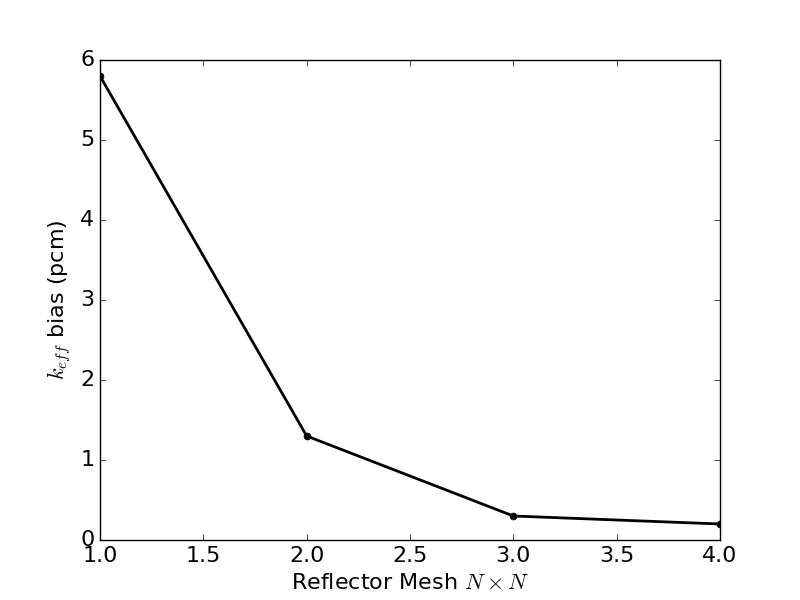
\includegraphics[width=0.7\linewidth]{figures/results/sensitivity/reflector_mesh_pcm.png}
	\caption[]{The bias in eigenvalue $k_{\textit{eff}}$ decreasing as reflector mesh of square discretization $N \times N$, where $N$ is the number of mesh discretizations in each pin-cell width, is refined within the radial water reflector.}
	\label{fig:rad-ref-pcm}
\end{figure}
\begin{figure}[h!]
	\centering
	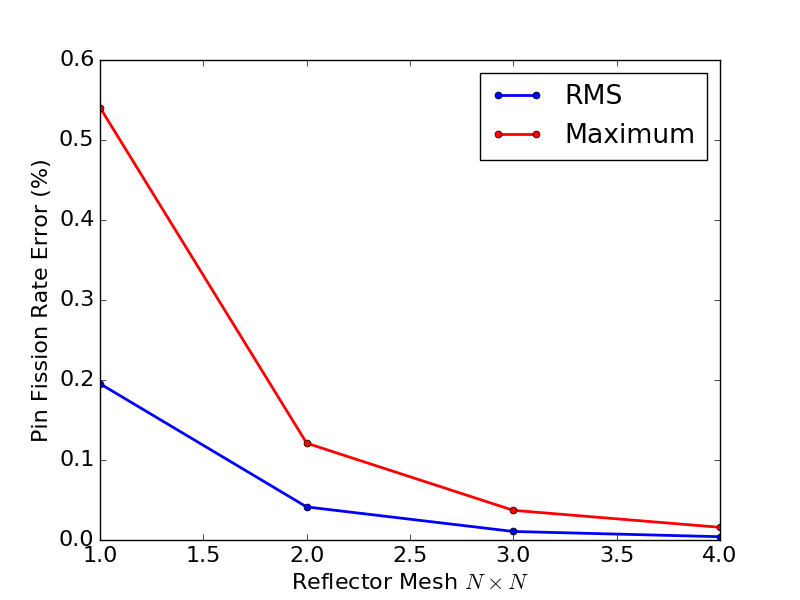
\includegraphics[width=0.7\linewidth]{figures/results/sensitivity/reflector_mesh_fr.png}
	\caption[]{The relative pellet-wise fission rate error decreasing as reflector mesh of square discretization $N \times N$, where $N$ is the number of mesh discretizations in each pin-cell width, is refined within the radial water reflector.}
	\label{fig:rad-ref-fr}
\end{figure}

A depiction of the mesh refinement of a cutout encompassing both core and reflector regions is shown in Figure~\ref{fig:moc-mesh-combined}. The left side of the illustration shows the discretization of the core, in which pin-cells are carved into sectors. The baffle and water reflector on the right side are cut into rectangular regions formed by the superposition of material boundaries and the uniform mesh overlay.

\begin{figure}[h!]
	\centering
	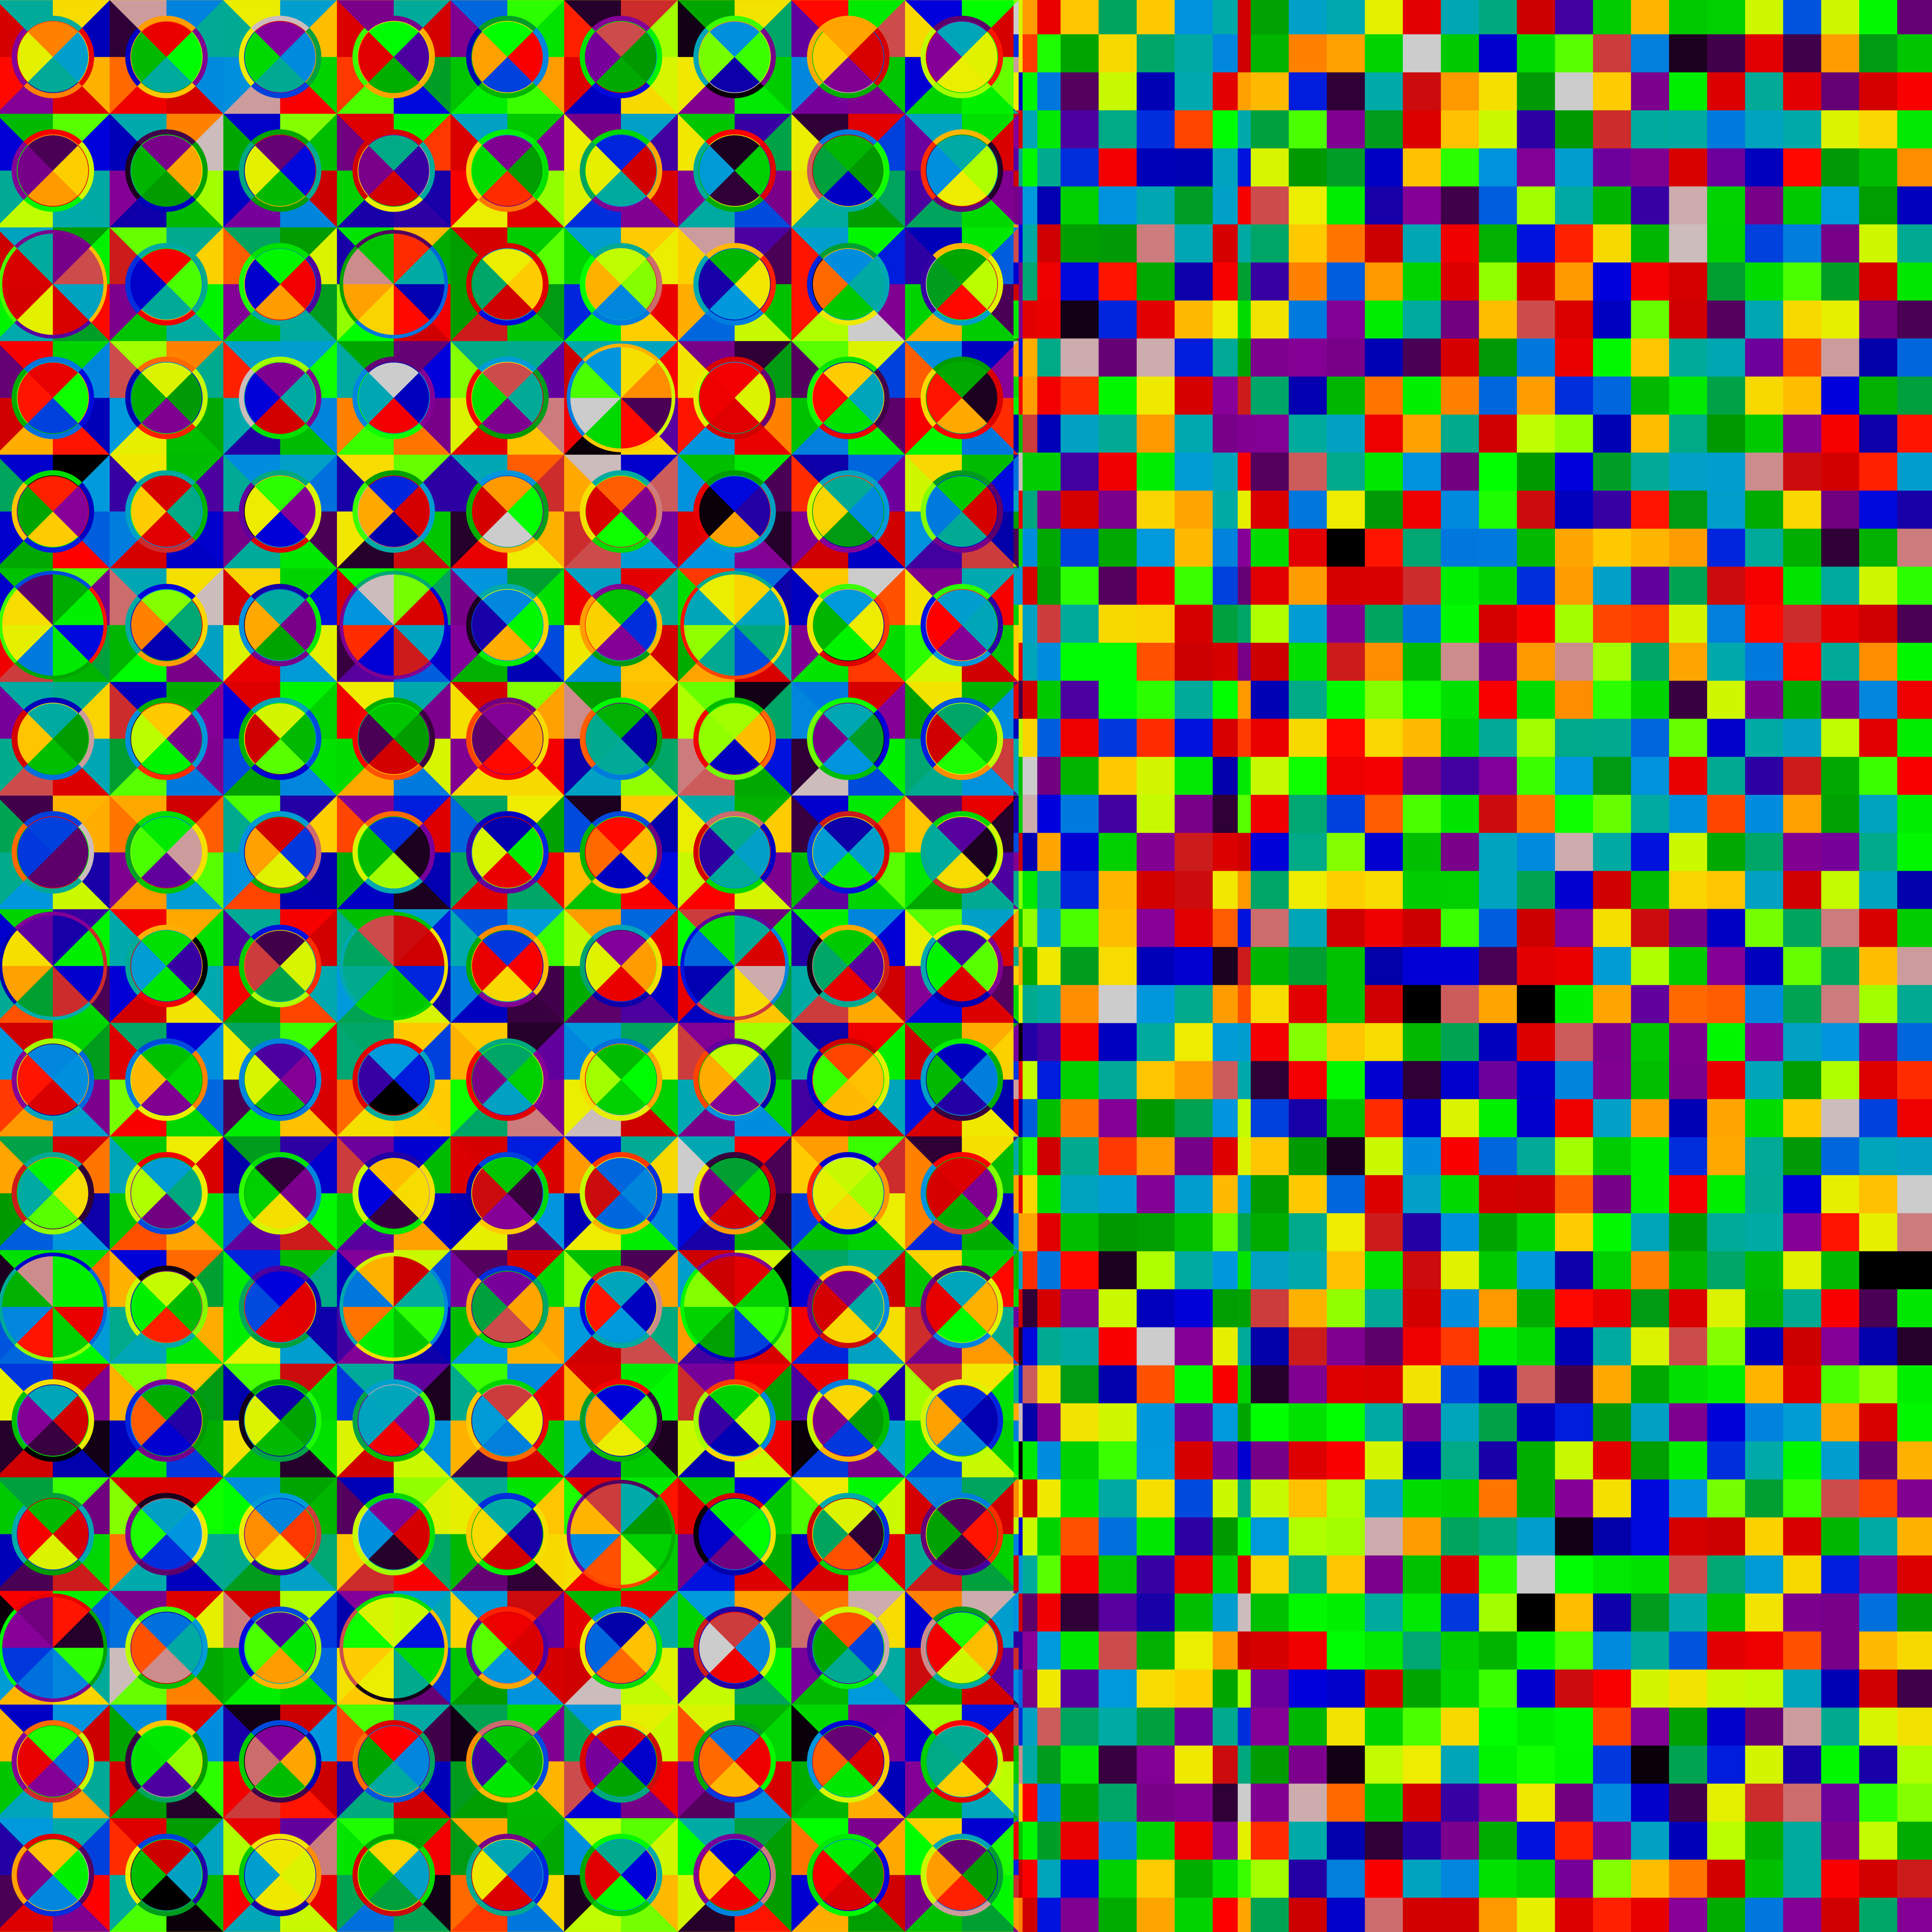
\includegraphics[width=0.7\linewidth]{figures/moc-mesh-combined.png}
	\caption[]{The chosen radial mesh refinement depicted near the periphery of the core, illustrating both core and reflector mesh.}
	\label{fig:moc-mesh-combined}
\end{figure}

\newpage
\subsection{Radial Ray Refinement}

Next, the \ac{MOC} radial ray parameters are investigated. The single assembly model is used in these tests, as described in Appendix~\ref{app:beavrs-single-assembly}. This model has full axial height and includes grid spacers and axial water reflectors. For the radial discretization, the previous studies are used to inform the selected parameters, as given in Table~\ref{tab:rad-ray-ref-params}. The number of azimuthal angles in $[0, 2\pi]$ and radial ray spacing required for accurate simulations are then tested using these assumed parameters. The radial mesh in the upper and lower water reflectors follows the same discretization present within the core. The radial profile of the fission rate distribution is very similar to the short assembly model, shown in Figure~\ref{fig:short-assembly-radial}.

\begin{table}[ht]
	\centering
	\caption{MOC ray and mesh parameters for radial ray refinement studies}
	\medskip
	\begin{tabular}{lc}
		\hline
		Number of Fuel Sectors & 4 \\
		Number of Guide Tube Sectors & 8 \\
		Number of Moderator Sectors & 8 \\
		Axial Ray Spacing & 0.75 cm \\
		Number of Polar Angles & 10 \\
		Axial Source Height & 2.0 cm \\
		\hline
	\end{tabular}
	\label{tab:rad-ray-ref-params}
\end{table}

\subsubsection{Radial Ray Spacing Sensitivity}

First, the radial ray spacing is tested. In these tests, the number of azimuthal angles is chosen to be 32. This is a factor of 2 away from the expected parameter, but still reasonably fine so it is assumed the radial ray spacing sensitivity is not significantly altered. The results of the sensitivity study are presented in Figures~\ref{fig:radial-rs-pcm} and \ref{fig:radial-rs-fr} for eigenvalue and fission rate, respectively. All errors and biases are reported relative to the case with 0.0125 cm radial ray spacing. These results show the expected radial ray spacing of 0.05 cm is sufficient to achieve less than 0.1\% maximum pellet-wise fission rate error and less than 5 pcm bias.

\begin{figure}[h!]
	\centering
	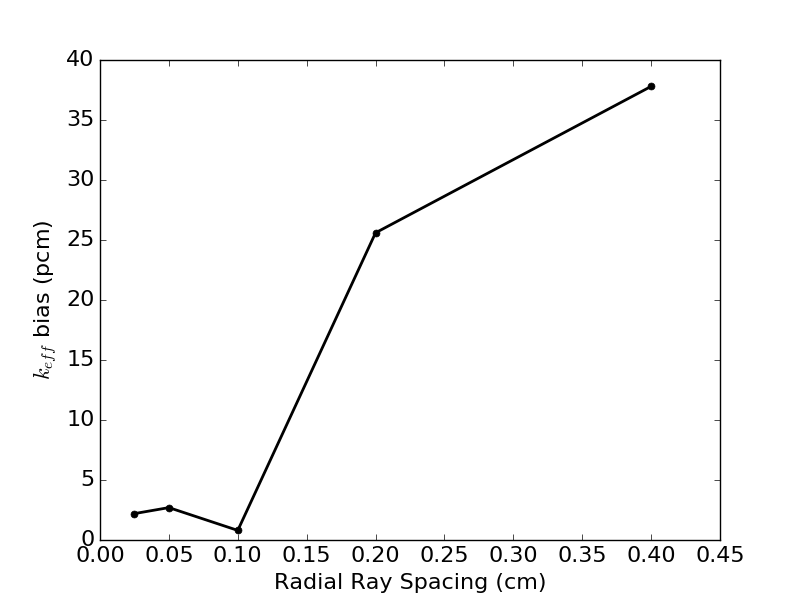
\includegraphics[width=0.7\linewidth]{figures/results/sensitivity/rad_spacing_pcm.png}
	\caption[]{The bias in eigenvalue $k_{\textit{eff}}$ decreasing as radial ray spacing is refined.}
	\label{fig:radial-rs-pcm}
\end{figure}
\begin{figure}[h!]
	\centering
	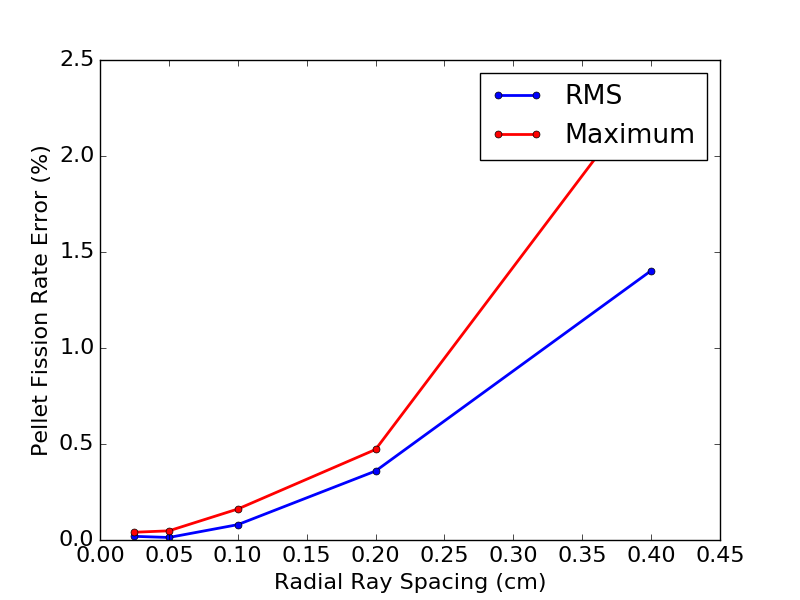
\includegraphics[width=0.7\linewidth]{figures/results/sensitivity/rad_spacing_fr_new.png}
	\caption[]{The relative pellet-wise fission rate error decreasing as radial ray spacing is refined.}
	\label{fig:radial-rs-fr}
\end{figure}

\newpage
\subsubsection{Azimuthal Angle Sensitivity}

The number of azimuthal angles is the last radial parameter to be tested. For these studies the radial ray spacing is chosen to be 0.1 cm, again a factor of 2 coarser than the expected parameter. The results of the sensitivity study are presented in Figures~\ref{fig:az-angles-pcm} and \ref{fig:az-angles-fr} for eigenvalue and fission rate, respectively. All errors and biases are reported relative to the case with 256 azimuthal angles.

\begin{figure}[h!]
	\centering
	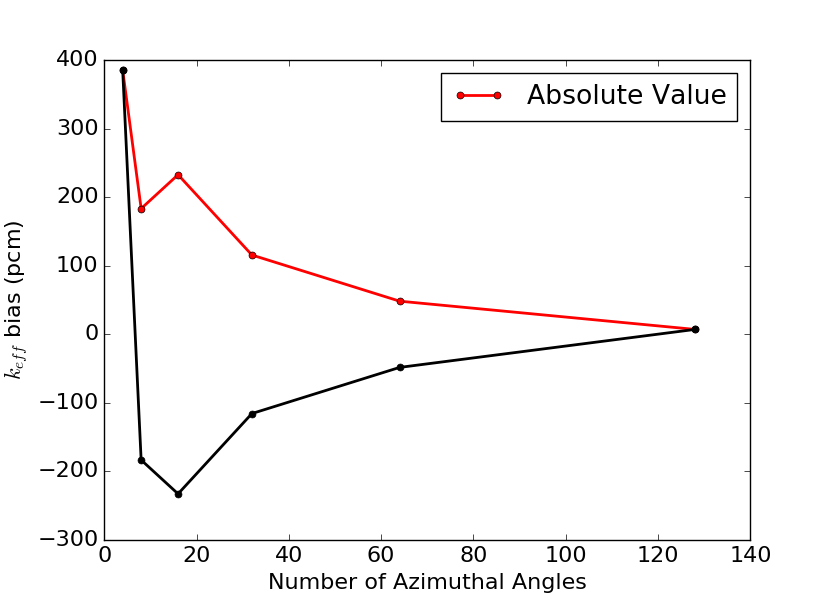
\includegraphics[width=0.7\linewidth]{figures/results/sensitivity/az_angles_pcm.png}
	\caption[]{The bias in eigenvalue $k_{\textit{eff}}$ decreasing as the number of azimuthal angles is increased.}
	\label{fig:az-angles-pcm}
\end{figure}
\begin{figure}[h!]
	\centering
	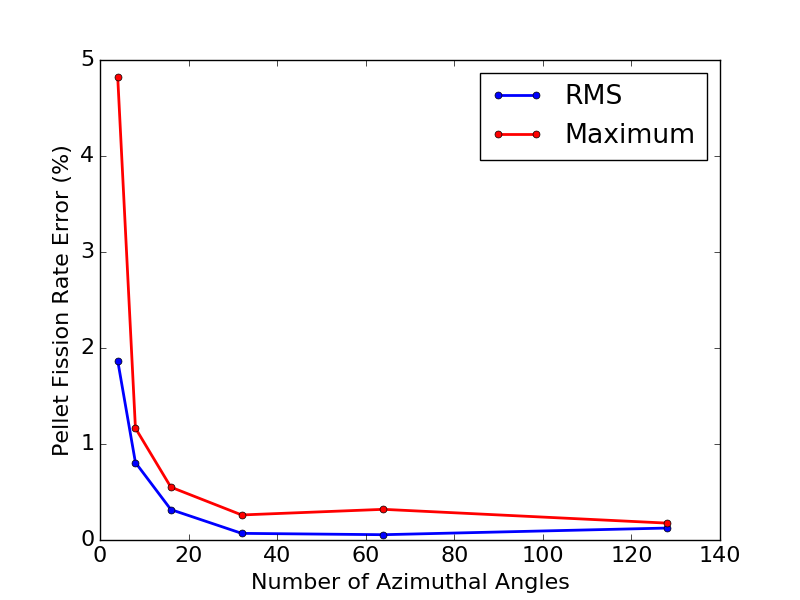
\includegraphics[width=0.7\linewidth]{figures/results/sensitivity/az_angles_fr_new.png}
	\caption[]{The relative pellet-wise fission rate error decreasing as the number of azimuthal angles is increased.}
	\label{fig:az-angles-fr}
\end{figure}

Here there seems to be significant sensitivity to the number of azimuthal angles. At the expected 64 azimuthal angles in $[0, 2\pi]$, there is a 48.3 pcm bias. However, the error in pellet-wise reaction rates is significantly less with the 64 azimuthal angle case producing less than 0.1\% \ac{RMS} error and less than 0.5\% maximum error. Therefore, the expected 64 azimuthal angles are assumed to be sufficient for accurately resolving the fission rate distribution. 

\section{Axial Sensitivity}
\label{sec:axial-sensitivity}

The previous section studied radial sensitivities, which are known quite well due to extensive experience with 2D \ac{MOC}. Therefore, the studies were a verification that the expected parameters were sufficient to accurately simulate typical geometries and materials found in \acp{PWR}. 

In this section, the axial sensitivities are studied, for which there is much less collective experience. 3D \ac{MOC} solvers have only recently been investigated in great detail. Therefore, rather than verifying a set of \ac{MOC} parameters to be sufficient for accurate simulations, a search is required to find the accurate parameters. This requires some metric for determining whether a simulation is sufficiently accurate.

The following criteria is selected to constitute an accurate simulation: less than 1.0\% \ac{RMS} pellet fission rate error, less than 3.0\% maximum pellet fission rate error, and less than 20 pcm bias on eigenvalue compared with a converged reference solution. The pellet fission rate is defined to be the fission rate within a given 2.0 cm tall fuel pin region. The reference solution for every case is chosen by further refining the parameter of interest, similar to the radial studies. This allows each parameter to be independently studied.

In this study, the single assembly model detailed in Appendix~\ref{app:beavrs-single-assembly} is chosen which contains axial water reflectors and grid spacers. It does not contain any inserted rods. Later, a single assembly with inserted rods is analyzed to determine the \ac{MOC} parameters when there are significant axial gradients. The axial profile of the fission distribution for the single assembly model without rod insertions is presented in Figure~\ref{fig:single-assembly-axial}, formed from an OpenMOC run with fine \ac{MOC} parameters and radially integrating fission rates. Notice the fission distribution dips around grid spacers.

\begin{figure}[h!]
	\centering
	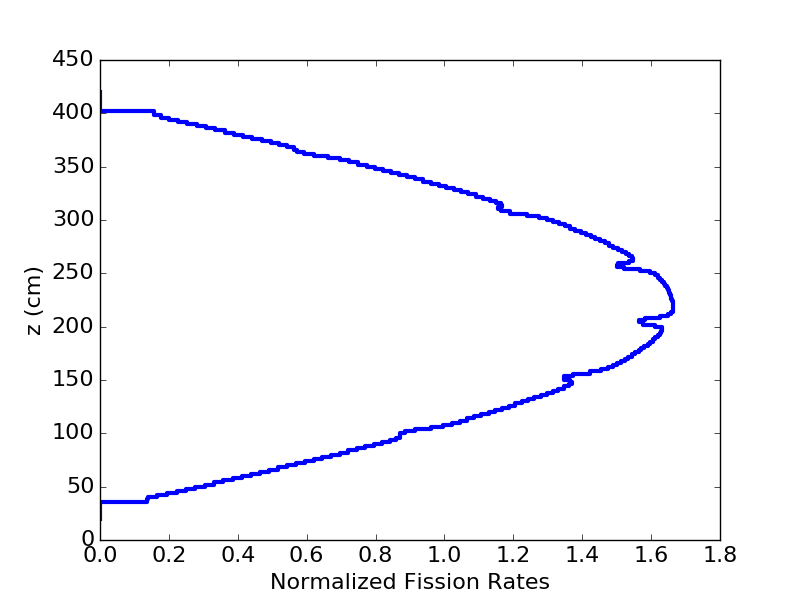
\includegraphics[width=0.7\linewidth]{figures/results/rr-plots/single-assembly-axial.png}
	\caption[]{The axial fission rate distribution of the single assembly model formed from radially integrating reaction rates in each 2 cm tall region.}
	\label{fig:single-assembly-axial}
\end{figure}

This section focuses on understanding the sensitivity to three axial parameters: the axial source height, the axial ray spacing, and the number of polar angles in $[0, \pi]$. For the axial source height sensitivity tests, a uniform axial mesh is imposed in order to simplify the study. Due to the structure of the test geometries presented in Appendix~\ref{app:beavrs}, all material boundaries occur at even intervals. Therefore, to impose a uniform axial mesh, the maximum axial source height is 2.0 cm. The axial ray spacing and polar angle tests are conducted in a similar fashion to the radial ray spacing and azimuthal angle sensitivity tests. For all tests, the radial parameters presented in Table~\ref{tab:axial-test-radial-params} are used. The radial mesh in the axial water reflectors follows the same discretization as that present within the core.

\begin{table}[ht]
	\centering
	\caption{MOC ray and mesh parameters for radial ray refinement studies}
	\medskip
	\begin{tabular}{lc}
		\hline
		Number of Fuel Sectors & 4 \\
		Number of Guide Tube Sectors & 8 \\
		Number of Moderator Sectors & 8 \\
		Number of Azimuthal Angles & 32 \\
		Radial Ray Spacing & 0.1 cm \\
		\hline
	\end{tabular}
	\label{tab:axial-test-radial-params}
\end{table}

\subsection{Axial Source Height Sensitivity}
\label{sec:axial-source-height-sensitivity}

First, the axial source height sensitivity study is conducted. For these tests, 10 polar angles and an axial ray spacing of 0.09375 cm (3/32 cm) are selected. The reference case has an axial source height of 0.25 cm. The results are presented in Figures~\ref{fig:axial-sh-pcm} and \ref{fig:axial-sh-fr} for eigenvalue and fission rate, respectively. 

\begin{figure}[h!]
	\centering
	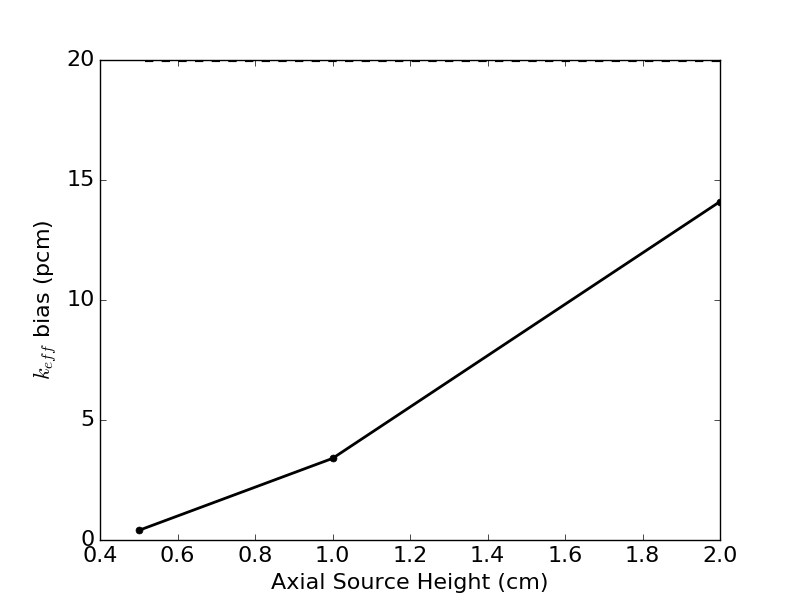
\includegraphics[width=0.65\linewidth]{figures/results/sensitivity/source_height_pcm.png}
	\caption[]{The bias in eigenvalue $k_{\textit{eff}}$ decreasing as axial source height is refined.}
	\label{fig:axial-sh-pcm}
\end{figure}
\begin{figure}[h!]
	\centering
	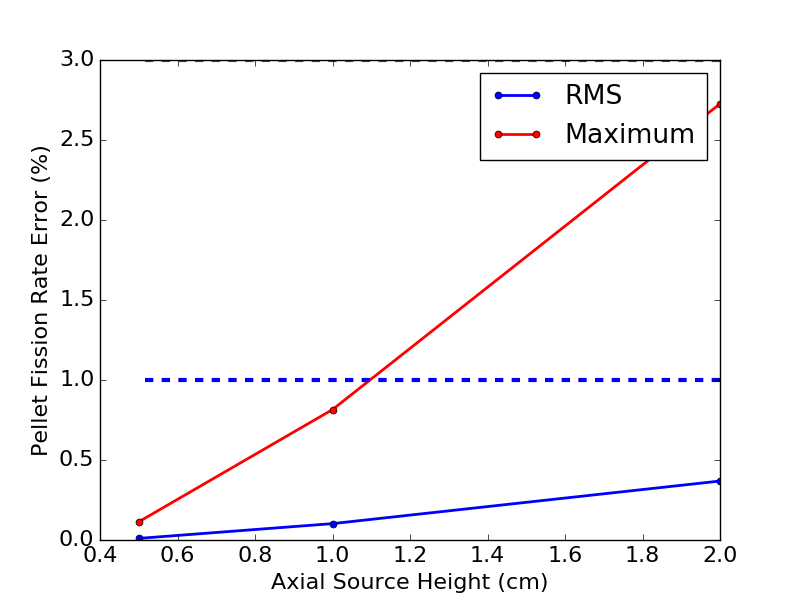
\includegraphics[width=0.65\linewidth]{figures/results/sensitivity/source_height_fr.png}
	\caption[]{The relative pellet-wise fission rate error decreasing as axial source height is refined.}
	\label{fig:axial-sh-fr}
\end{figure}

Notice that there is a sensitivity to axial source height but with 2.0 cm source height, the accuracy criteria is satisfied. However, if less than 1.0\% \textit{maximum} fission rate error were required, the axial source height would need to be 1.0 cm.

\subsection{Axial Ray Spacing Sensitivity}
\label{sec:axial-ray-spacing-sensitivity}

Next, the axial ray spacing sensitivity is studied. For these tests, 10 polar angles and an axial source height of 2.0 cm are selected. Since, the axial ray spacing should be less than the axial source height to ensure at least one crossing of each source region per angle, the coarsest axial ray spacing is chosen to be 1.5 cm. Then the ray spacing is halved each time the ray spacing is refined. The reference is chosen to be 0.09375 cm (3/32 cm). The results are presented in Figures~\ref{fig:axial-sh-pcm} and \ref{fig:axial-sh-fr} for eigenvalue and fission rate, respectively. These results show that 1.5 cm axial ray spacing is sufficient to satisfy the accuracy criteria. However, if less than 1.0\% maximum fission rate error is required, the axial ray spacing would need to be 0.75 cm.

\begin{figure}[h!]
	\centering
	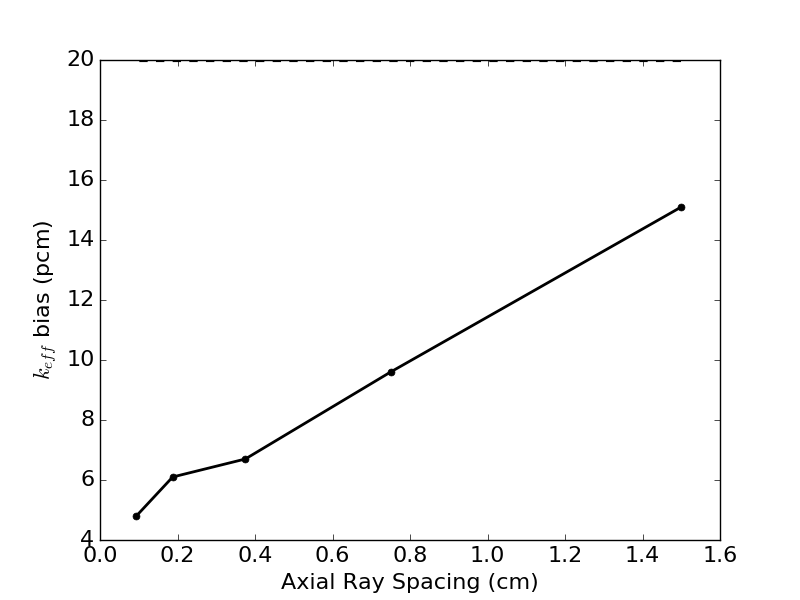
\includegraphics[width=0.7\linewidth]{figures/results/sensitivity/z_spacing_pcm.png}
	\caption[]{The bias in eigenvalue $k_{\textit{eff}}$ decreasing as axial ray spacing is refined.}
	\label{fig:axial-rs-pcm}
\end{figure}
\begin{figure}[h!]
	\centering
	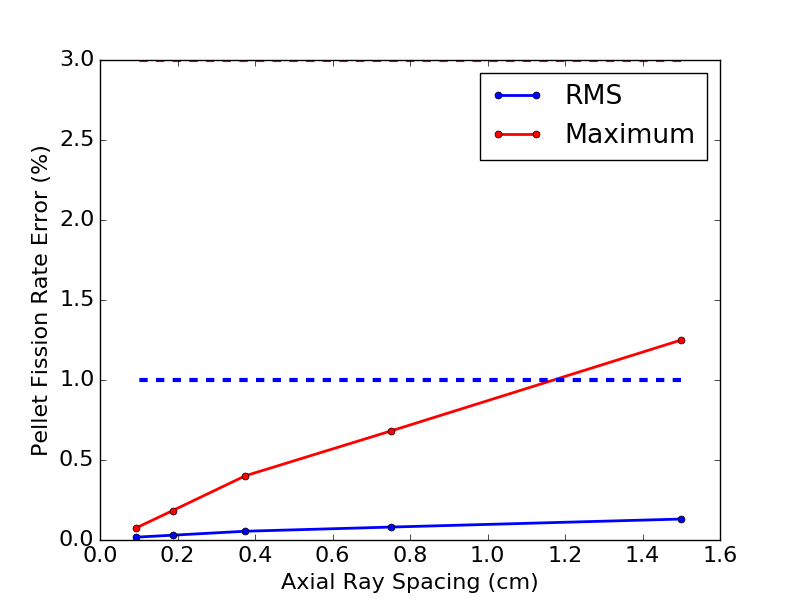
\includegraphics[width=0.7\linewidth]{figures/results/sensitivity/z_spacing_fr.png}
	\caption[]{The relative pellet-wise fission rate error decreasing as axial ray spacing is refined.}
	\label{fig:axial-rs-fr}
\end{figure}

This result is quite similar to the axial source height sensitivity whereby a refinement of the parameter may be useful. Since it is not possible to refine axial source height further with an axial ray spacing of 1.5 cm while ensuring each axial source region is traversed, the axial ray spacing is chosen to be 0.75 cm to allow for a source height refinement if necessary.

\subsection{Polar Angle Sensitivity}
\label{sec:polar-angle-sensitivity}

Lastly, the polar angle sensitivity study is conducted using an axial ray spacing of 0.25 cm and an axial source height of 2.0 cm. This fine axial ray spacing allows the trend to be less sensitive to small perturbations in track laydown when changing polar angles, causing the trend to be more directly visible. All results use the Gauss-Legendre polar quadrature. The reference is chosen to be 32 polar angles in $[0, \pi]$. The results are presented in Figures~\ref{fig:polar-angles-pcm} and \ref{fig:polar-angles-fr} for eigenvalue and fission rate, respectively. These results show that only 6 polar angles are necessary to achieve the accuracy criteria. However, 2D \ac{MOC} simulations with Gauss-Legendre quadrature typically use a minimum of 5 polar angles in $[0,\pi/2]$, equivalent to 10 polar angles for 3D \ac{MOC} in $[0,\pi]$. Therefore, 10 polar angles are assumed to be necessary.

\begin{figure}[h!]
	\centering
	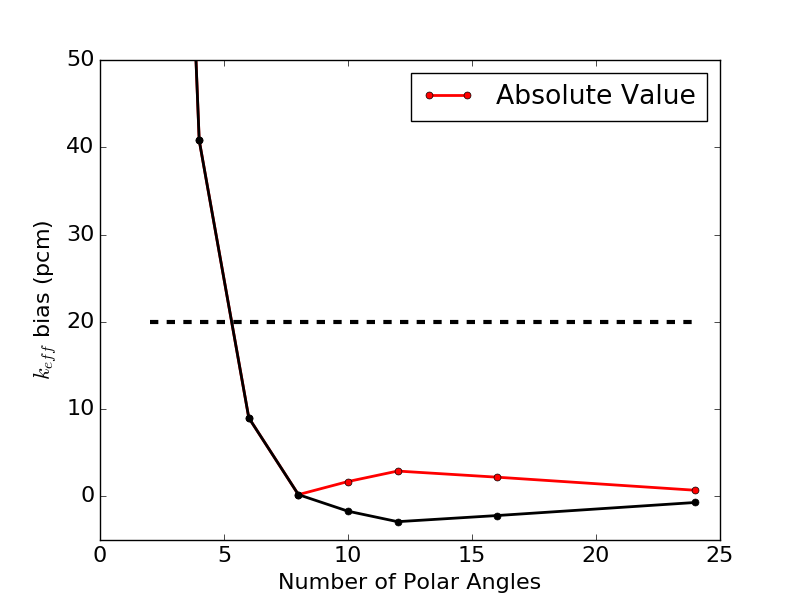
\includegraphics[width=0.7\linewidth]{figures/results/sensitivity/polar_angles_pcm.png}
	\caption[]{The bias in eigenvalue $k_{\textit{eff}}$ decreasing as the number of polar angles is increased.}
	\label{fig:polar-angles-pcm}
\end{figure}
\begin{figure}[h!]
	\centering
	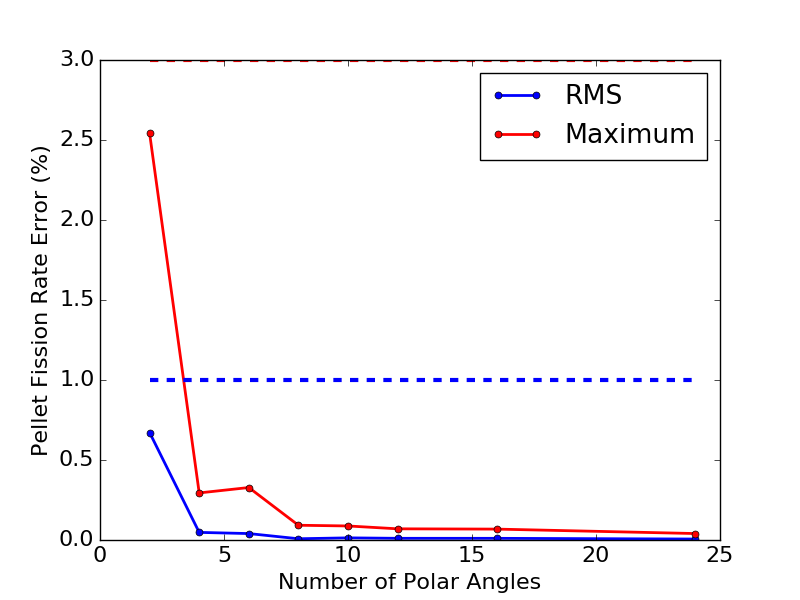
\includegraphics[width=0.7\linewidth]{figures/results/sensitivity/polar_angles_fr.png}
	\caption[]{The relative pellet-wise fission rate error decreasing as the number of polar angles is increased.}
	\label{fig:polar-angles-fr}
\end{figure}


\newpage
\section{Axial Sensitivity on a Rodded Assembly}
\label{sec:axial-sensitivity-rodded}

In the previous section, the axial \ac{MOC} parameters were studied for a single assembly problem with no control rod insertions, allowing for smooth axial gradients. When control rods are inserted, the gradients can become significant. To observe this effect, the rodded single assembly model discussed in Appendix~\ref{app:rodded-single-assembly} is selected. In this problem, a rod is halfway inserted into the assembly, creating a significant distortion in the power profile. The axial profile of this model is presented in Figure~\ref{fig:single-assembly-rodded-axial}, again formed from an OpenMOC run with fine \ac{MOC} parameters and radially integrating fission rates.

\begin{figure}[h!]
	\centering
	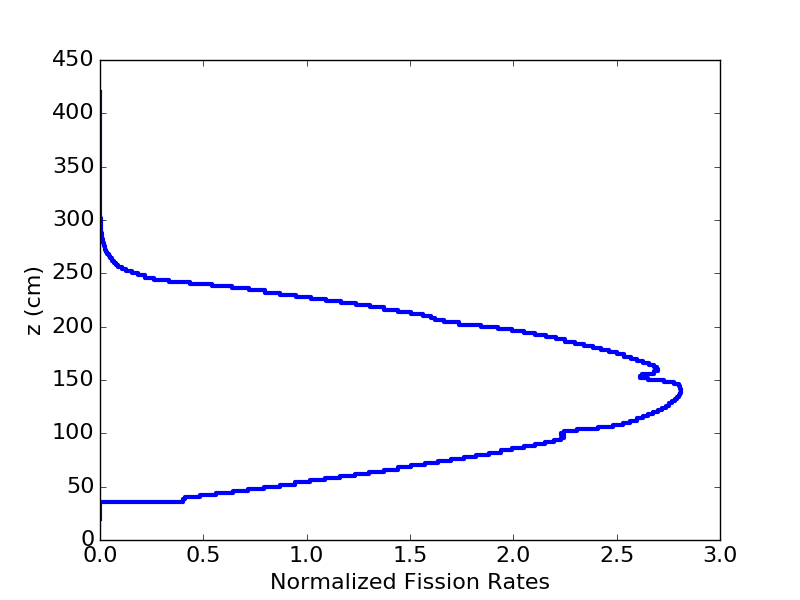
\includegraphics[width=0.7\linewidth]{figures/results/rr-plots/single-assembly-rodded-axial.png}
	\caption[]{The axial fission rate distribution of the rodded single assembly model formed from radially integrating reaction rates in each 2 cm tall region.}
	\label{fig:single-assembly-rodded-axial}
\end{figure}

The presence of significant gradients mean finer axial parameters may be required. Therefore, the axial sensitivity study is repeated for the rodded single assembly test problem. Again, the radial parameters described in Table~\ref{tab:axial-test-radial-params} are selected. Since the fission distribution drops significantly past the control rod tip, fission rate error comparisons in this section only consider the region below the axial height of 250 cm.

\subsection{Axial Source Height Sensitivity}

First, the axial source height is again analyzed using 10 polar angles and an axial ray spacing of 0.09375 cm. The reference again has 0.25 cm axial source height. The results are presented in Figures~\ref{fig:polar-angles-pcm} and \ref{fig:polar-angles-fr} for eigenvalue and fission rate, respectively. Now, a finer axial source discretization is required, with a source height of 1.0 cm necessary to achieve the accuracy criteria.

\begin{figure}[h!]
	\centering
	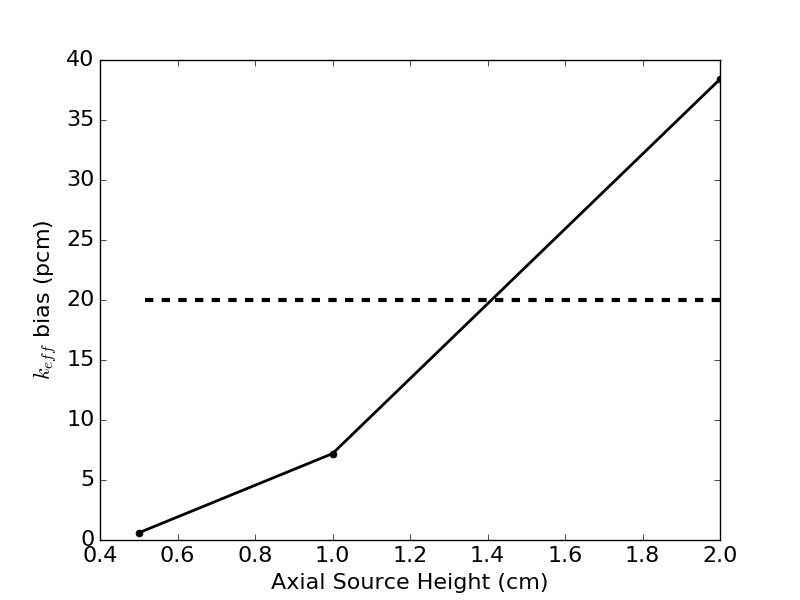
\includegraphics[width=0.7\linewidth]{figures/results/sensitivity/rodded_source_height_pcm.png}
	\caption[]{The bias in eigenvalue $k_{\textit{eff}}$ decreasing as axial source height is refined.}
	\label{fig:rodded-axial-sh-pcm}
\end{figure}
\begin{figure}[h!]
	\centering
	\includegraphics[width=0.7\linewidth]{figures/results/sensitivity/rodded_source_height_fr_new.png}
	\caption[]{The relative pellet-wise fission rate error decreasing as axial source height is refined.}
	\label{fig:rodded-axial-sh-fr}
\end{figure}

\subsection{Axial Ray Spacing Sensitivity}

Next, the axial ray spacing is analyzed using 10 polar angles and a source height of 0.5 cm. The reference is chosen to have 0.023 cm (3/128 cm) axial ray spacing. Since the source height has been decreased from 2.0 cm to 0.5 cm in comparison with the tests in Section~\ref{sec:axial-ray-spacing-sensitivity}, the coarsest axial ray spacing present in the previous tests that still traverses every axial source region is 0.375 cm (3/8 cm). Again, the axial ray spacing is halved each time the ray spacing is refined. The results are presented in Figures~\ref{fig:rodded-axial-rs-pcm} and \ref{fig:rodded-axial-rs-fr} for eigenvalue and fission rate, respectively. An axial ray spacing of 0.375 cm (3/16 cm) is sufficient to achieve less than 1\% maximum fission rate error.

\begin{figure}[h!]
	\centering
	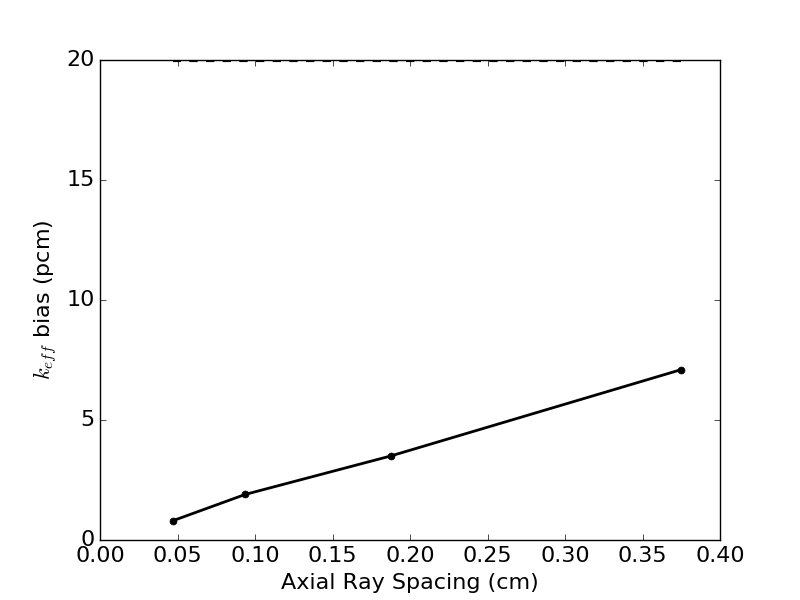
\includegraphics[width=0.7\linewidth]{figures/results/sensitivity/rodded_z_spacing_pcm.png}
	\caption[]{The bias in eigenvalue $k_{\textit{eff}}$ decreasing as axial ray spacing is refined.}
	\label{fig:rodded-axial-rs-pcm}
\end{figure}
\begin{figure}[h!]
	\centering
	\includegraphics[width=0.7\linewidth]{figures/results/sensitivity/rodded_z_spacing_fr_new.png}
	\caption[]{The relative pellet-wise fission rate error decreasing as axial ray spacing is refined.}
	\label{fig:rodded-axial-rs-fr}
\end{figure}

\subsection{Polar Angle Sensitivity}

Lastly, the polar angle sensitivity is conducted with the same parameters as the case without rod insertions in Section~\ref{sec:polar-angle-sensitivity}: 0.25 cm axial ray spacing and 2.0 cm axial source height. Again, the reference is 32 polar angles. While the axial source height is coarser than necessary to accurately converge the problem, it is assumed that the sensitivity is similar with the necessary parameter. The results are presented in Figures~\ref{fig:rodded-axial-rs-pcm} and \ref{fig:rodded-axial-rs-fr} for eigenvalue and fission rate, respectively, showing very little difference from the case without rod insertions. Again, 6 polar angles are sufficient to meet the criteria but 10 polar angles are selected due to the 2D~\ac{MOC} considerations outlined in Section~\ref{sec:polar-angle-sensitivity}.

\begin{figure}[h!]
	\centering
	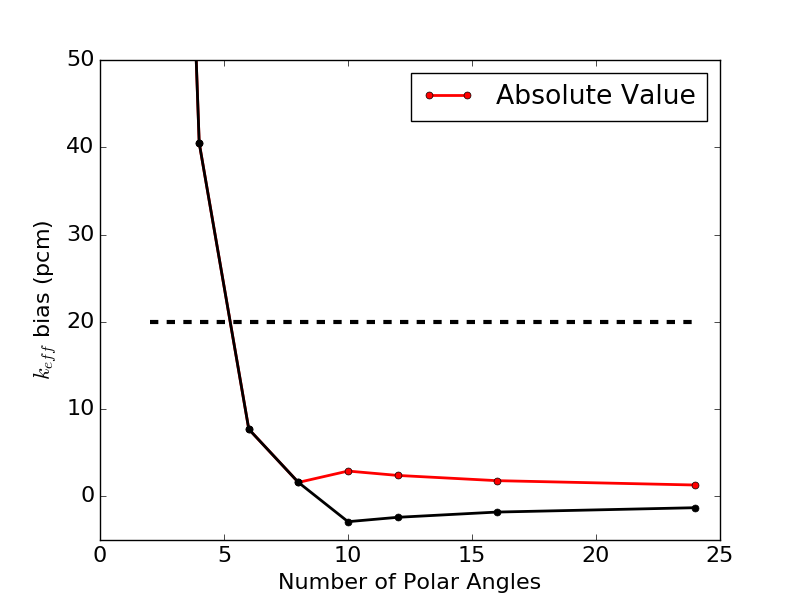
\includegraphics[width=0.7\linewidth]{figures/results/sensitivity/rodded_polar_angles_pcm.png}
	\caption[]{The bias in eigenvalue $k_{\textit{eff}}$ decreasing as the number of polar angles is increased.}
	\label{fig:rodded-polar-angles-pcm}
\end{figure}
\begin{figure}[h!]
	\centering
	\includegraphics[width=0.7\linewidth]{figures/results/sensitivity/rodded_polar_angles_fr_new.png}
	\caption[]{The relative pellet-wise fission rate error decreasing as the number of polar angles is increased.}
	\label{fig:rodded-polar-angles-fr}
\end{figure}

\newpage
\section{Comparison with Flat Source MOC}
\label{sec:flat-linear-comparison}

In the previous sections, the radial and axial parameters required to achieve accurate 3D \ac{MOC} solutions were investigated. In this section, the parameters which were found to be sufficient in accurately simulation \ac{PWR} problems -- and presented later during the conclusion in Table~\ref{tab:final-params} -- are used to simulate the single assembly model described in Appendix~\ref{app:beavrs-single-assembly} for both linear source and flat source solvers. Since the parameters were derived with the linear source parameters, there should be some bias introduced with the flat source solver.

The results show a bias of 41 pcm was incurred with the flat source solver compared with the linear source solution. Additionally, the pellet-wise \ac{RMS} relative fission rate difference was 2.1\% and the maximum relative fission rate difference was 12.9\%. 

A reference OpenMC solution was generated for the problem to compare the accuracy of flat and linear solutions. The reference OpenMC results simulated 400 batches of neutrons (300 inactive, 100 active) with $10^7$ particles per batch on the single assembly model. The axial fission rate error relative to the OpenMC reference solution is presented in Figure~\ref{fig:fs-ls-axial-error} where the fission rates in each axial interval are formed by radially integrating all region-wise fission rates within the axial interval.

\begin{figure}[h!]
	\centering
	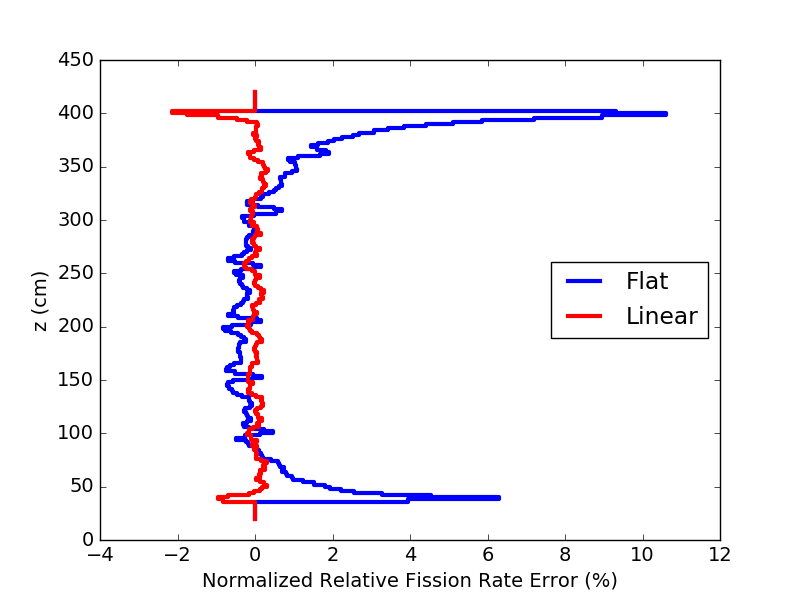
\includegraphics[width=0.7\linewidth]{figures/results/error-plots/sa_fs_ls_axial_error.png}
	\caption[]{The axial fission rate error of flat source and linear source simulations relative to an OpenMC reference solution on the single assembly test problem.}
	\label{fig:fs-ls-axial-error}
\end{figure}

From the axial fission rate error distribution in Figure~\ref{fig:fs-ls-axial-error}, the largest errors occur near the axial water reflectors. This is due to the flat source approximation not being able to capture the strong axial gradients that occur near the reflectors. In order to achieve comparable accuracy using the flat source solver, a significantly finer source discretization in the axial direction would likely need to be used, causing the axial ray spacing to also be further refined. 

\section{CMFD Acceleration}
\label{sec:cmfd-convergence-params}

In all of the previous sections of this chapter, only solution accuracy was investigated as a function of \ac{MOC} parameters. \ac{CMFD} acceleration is often necessary to achieve reasonable convergence rates, as detailed in Appendix~\ref{app:cmfd-acceleration}. Therefore, the sensitivity of convergence rate to \ac{CMFD} parameters is discussed in this chapter. It is important to note that the acceleration does not impact solution accuracy.

\ac{CMFD} is implemented in OpenMOC with uniform mesh on any reduced group structure. Therefore, the important parameters for defining \ac{CMFD} acceleration are the mesh dimensions and the number of energy groups. For the \ac{PWR} problems investigated in this thesis, pin-cell mesh is always chosen in the radial plane. This is chosen based on extensive experience in 2D \ac{MOC}. Therefore, this section focuses on understanding the sensitivity to two remaining parameters: the axial mesh and the number of energy groups used in the \ac{CMFD} solver. In order to decrease run-time requirements of the \ac{CMFD} solver, the parameters should be chosen to be as coarse as possible while maintaining an optimal convergence rate.

For this investigation, the single assembly model described in Appendix~\ref{app:beavrs-single-assembly} is used with the \ac{MOC} parameters determined in the previous sections to obtain reasonable solution accuracy, presented later in Table~\ref{tab:final-params}. For all the trials, \ac{MOC} diagonal damping is applied, as discussed in Chapter~\ref{chap:moc-convergence}, with $\rho = 1/4$. A \ac{CMFD} damping factor of 0.7 is also applied for all trials.

\subsection{Axial Mesh Sensitivity}
First, the axial mesh sensitivity is investigated. Since a uniform mesh is required by the \ac{CMFD} solver, the number of axial \ac{CMFD} cells $N_Z$ uniquely defines the axial mesh. The axial height of the single assembly problem is 400 cm and the axial source height is 2.0 cm. When \ac{CMFD} boundaries intersect source regions, the source regions are split such that each source region belongs to uniquely one \ac{CMFD} cell. Therefore, in order to have the same source region discretization for all tested cases, the number of axial cells $N_Z$ is chosen such that $200 / N_Z$ is an integer. The convergence results are presented in Figure~\ref{fig:cmfd-axial-cells} for a variety of \ac{CMFD} axial mesh cells. 

\begin{figure}[h!]
	\centering
	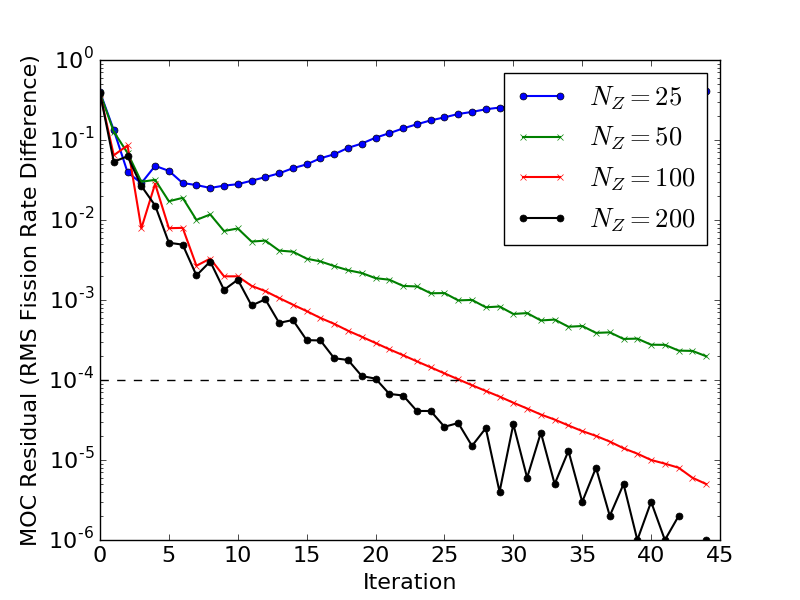
\includegraphics[width=0.7\linewidth]{figures/results/sensitivity/cmfd-axial-cells.png}
	\caption[]{Convergence with a variety of \ac{CMFD} axial mesh cells, $N_Z$.}
	\label{fig:cmfd-axial-cells}
\end{figure}

The results show that further mesh discretization improves convergence rate all the way to the maximum number of axial \ac{CMFD} cells ($N_Z = 200$) in which each \ac{CMFD} spans only the height of one \ac{MOC} source region. Therefore, 200 \ac{CMFD} cells should be used in all calculations. At just 25 axial \ac{CMFD} cells, it is not clear that the solution will even converge, as the residual does not drop significantly in the first 50 iterations.

\newpage
\subsection{Energy Group Sensitivity}

Next, the sensitivity to the number of \ac{CMFD} energy groups is studied. Since the number of \ac{MOC} energy groups is 70, the maximum number of \ac{CMFD} groups is 70. For less than 70 energy groups, certain groups are combined. There are many configurations in which the group structure can be collapsed into a reduced \ac{CMFD} group structure. In OpenMOC, any collapse is possible, but the CASMO-4 group structures~\cite{edenius1995casmo} are implemented for convenience. These group structures can be found in Appendix~\ref{app:energy-groups}. Using these reduced group structures and varying the number of \ac{CMFD} groups $G_C$, the sensitivity of convergence rate to the \ac{CMFD} group structure is tested. The results are shown in Figure~\ref{fig:cmfd-energy-groups}.

\begin{figure}[h!]
	\centering
	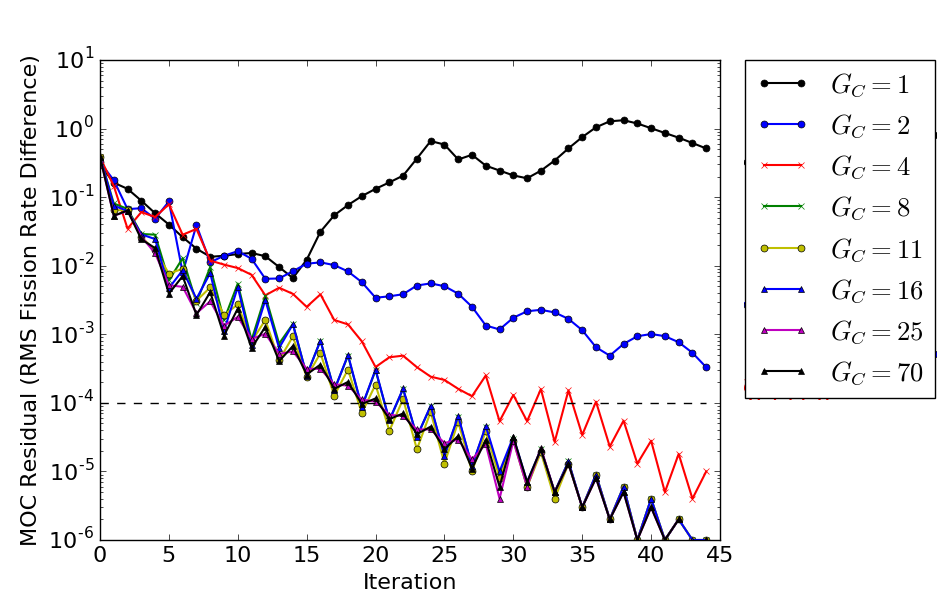
\includegraphics[width=0.9\linewidth]{figures/results/sensitivity/cmfd-groups.png}
	\caption[]{Convergence with a variety of \ac{CMFD} energy group structures with number of groups $G_C$.}
	\label{fig:cmfd-energy-groups}
\end{figure}

Notice that the convergence history is not significantly different for 8 or more \ac{CMFD} groups. However, when the number of \ac{CMFD} groups is reduced beyond 8, the convergence suffers. With one \ac{CMFD} group, the residual does not drop significantly during the first 50 iterations. Therefore, this study shows that 8 \ac{CMFD} groups should be used in simulation as it captures the optimal convergence rate with the minimum number of energy groups.

\section{Domain Decomposition}
\label{sec:domain-decomposition-convergence}

In Chapter~\ref{chap:domain-decomposition}, it was noted that domain decomposition could slow the convergence rate since angular fluxes are lagged at domain interfaces. Here, the sensitivity to axial domain decomposition is studied on a single assembly model. The \ac{MOC} and \ac{CMFD} parameters presented later during the conclusion in Table~\ref{tab:final-params} are used in this study, except the number of azimuthal angles is reduced to 32 and the radial ray spacing is coarsened to 0.1 cm in order to run in reasonable time without domain decomposition. The sensitivity of convergence to the number of axial domains $D_Z$ is shown in Figure~\ref{fig:axial-dd}.

\begin{figure}[h!]
	\centering
	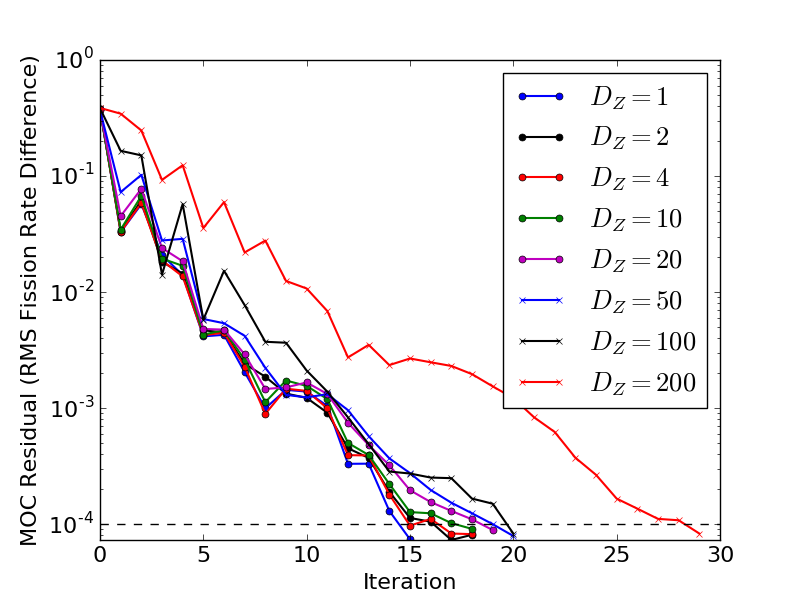
\includegraphics[width=0.9\linewidth]{figures/results/sensitivity/domains_z.png}
	\caption[]{Convergence with a $1 \times 1 \times D_Z$ domain decomposition used on the single assembly model.}
	\label{fig:axial-dd}
\end{figure}

The results show a slight but constant degradation in convergence rate as the assembly is decomposed into more axial domains up to 100 axial domains. At 200 axial domains, where each domain only covers one axial source region, the convergence rate is significantly degraded. However, a very fine axial decomposition is not intended. In order to most effectively reduce the memory storage per domain, nearly cubic domains should be created, as on-node computational work scales with domain volume but on-node memory storage scales with domain surface area. For the full core BEAVRS benchmark, a radial domain decomposition of single assemblies is intended, which have width approximately 21.42 cm. Since the height of the simulated BEAVRS model is 400 cm, an axial domain decomposition of 20 axial domains would lead to nearly cubic domains, and is the intended domain decomposition for the BEAVRS benchmark in this thesis. At 20 axial domains, the single assembly convergence is only slightly degraded from the single domain case. 


\section{Conclusion}
\label{sec:sensitivity-conclusion}

In this chapter, the sensitivity of solution accuracy to \ac{MOC} parameters was investigated in great detail. In addition, the convergence of \ac{CMFD} was studied as a function of \ac{CMFD} energy group structure and axial mesh. From these studies, the parameters given in Table~\ref{tab:final-params} are chosen to accurately and efficiently simulate \ac{PWR} problems using OpenMOC's 3D \ac{MOC} linear source solver. Using the flat source solver with these parameters incurs significant error.

\begin{table}[ht]
	\centering
	\caption{MOC ray and mesh parameters determined to accurately and efficiently simulate PWR problems}
	\medskip
	\begin{tabular}{lc}
		\hline
		Radial Ray Spacing & 0.05 cm \\
		Axial Ray Spacing & 0.75 cm \\
		Number of Azimuthal Angles & 64 \\
		Number of Polar Angles & 10 \\
		\hline
		Number of Fuel Sectors & 4 \\
		Number of Guide Tube Sectors & 8 \\
		Number of Moderator Sectors & 8 \\
		Axial Source Height & 2.0 cm \\
		Radial Reflector Mesh & $3\times 3$ cells per pin-cell mesh \\
		\hline
		\ac{CMFD} Cell Height & 2.0 cm \\
		Number of \ac{CMFD} Energy Groups & 8 \\
		\hline
	\end{tabular}
	\label{tab:final-params}
\end{table}

\vfill
\begin{highlightsbox}[frametitle=Highlights]
\begin{itemize}
  \item The presence of rod insertions requires axial source height and axial ray spacing to be refined, but there is little polar angle sensitivity.
  \item Significant error is introduced when the \ac{MOC} parameters necessary for accuracy with the linear source solver are used with the flat source \ac{MOC} solver
  \item For optimal \ac{CMFD} convergence, the \ac{CMFD} axial mesh should be the same as the \ac{MOC} axial mesh, but the number of \ac{CMFD} energy groups can be reduced to 8 from the 70 group \ac{MOC} structure without reduction in convergence rate
  \end{itemize}
\end{highlightsbox}
\vfill